\section{Slopes and Average Rates of Change}
\label{sec:slope}

\subsection{Precalculus Idea: Slope and Rate of Change}

% Start with an example.
\begin{wrapfigure}{R}{0.5\textwidth}
  \vspace{-20pt}
\centering
\begin{tikzpicture}[scale=1]
    \begin{axis}[
        date coordinates in=x,
        date ZERO=2019-12-31,
        ytick distance = 5,
        grid = both,
        major grid style = {gridGray},
        xticklabel = {\year-\month},
        ylabel = {Price ($\$10,000$)},
    ]
    \addplot[very thick, aldRed, mark=*] table[x=Date, y=Price] {datasets/bitcoin2020.dat};
    \end{axis}
\end{tikzpicture}
\caption{Price of Bitcoin in 2020, in Thousands of Dollars. Source: Coindesk; https://www.coindesk.com/price/bitcoin}
\label{fig:2-1-bitcoin2020}
\end{wrapfigure}
The price of an asset, such as a stock, commodity, or currency, relative to some other asset typically fluctuates in a chaotic manner. We can see if the price is increasing, decreasing, or relatively stable, in a qualitatative sense, by looking at a plot of the price of an asset over time. An example is the graph of the price of bitcoin\index{Bitcoin} during 2020. Figure \ref{fig:2-1-bitcoin2020} plots the price of bitcoin at the end of each month from December 2019 to December 2020. Suppose that we are interested in getting the average rate of change of this price over the course of the year. This calculation ignores are the intermediate fluctuations in price and just focuses on two values: the starting and ending prices. Note that price fluctuates by the second; we just plotted monthly data.

\begin{example}
Given that the price of one bitcoin was $\$7179.96$ at the end of 2019 and $\$29,111.52$ at the end of 2020, what was the average rate of change in the price of one bitcoin during 2020?

\solution In this context, the rate of change of the price is $\frac{\mbox{change in price}}{\mbox{change in time}}$. In many cases, the unit in the denominator is clear from context. In this case, the only unit of time that is given is years, but it would not be very illustrative to talk about the rate of change of the price in dollars per year if we only have a year's worth of data. In context, it makes more sense to talk about the rate of change per month or per day, for example. Recall that 2020 was a leap year, so there were 366 days.
\begin{align*}
\frac{\mbox{change in price}}{\mbox{change in time}} &= \frac{29111.52 - 7179.96 \mbox{ dollars}}{12 \mbox{ months}} = \$1827.63 \mbox{ per month} \\
&= \frac{29111.52 - 7179.96 \mbox{ dollars}}{366 \mbox{ days}} = \$59.9223 \mbox{ per day} \\
\end{align*}
Therefore, the price of one bitcoin changed at a rate of $\$1827.63$ per month, on average during 2020. We could also conclude that the price of one bitcoin increased at an average rate of $\$59.92$ per day in 2020.
\end{example}

\begin{wrapfigure}{R}{0.25\textwidth}
  \vspace{-20pt}
  \centering
    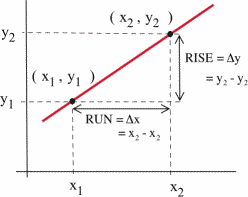
\includegraphics[width=0.24\textwidth]{img/chap2/image001.png}
  %\end{center}
%\vspace{-20pt}  
\caption{Slope between two points.}
\label{fig:2-slope}
\vspace{-10pt}
\end{wrapfigure}
The {\bf slope}\index{Slope} of a line measures how fast a line rises or falls as we move from left to right along the line. It measures the {\bf rate of change}\index{Rate of change} of the $y$-coordinate with respect to changes in the $x$-coordinate. If the line represents the distance an object traveled over time, for example, then the slope of the line represents the velocity of the object. In Figure \ref{fig:2-slope}, you can remind yourself how we calculate slope using two points on the line.

$$m = \mbox{Slope from } P \mbox{ to } Q = \frac{\mbox{rise}}{\mbox{run}} = \frac{y_2-y_1}{x_2-x_1} = \frac{\Delta y}{\Delta x}$$


\begin{wrapfigure}{R}{0.25\textwidth}
  \vspace{-10pt}
  \centering
    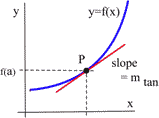
\includegraphics[width=0.24\textwidth]{img/chap2/image002.png}
  %\end{center}
%\vspace{-20pt}  
\caption{Tangent Line}
\label{fig:2-1-slopeCurve}
\vspace{-10pt}
\end{wrapfigure}

We would like to get that same kind of information (how fast the curve rises or falls, velocity from distance) even if the graph is not a straight line. But what happens if we try to find the slope of a curve\index{Slope!curve}, as in Figure \ref{fig:2-1-slopeCurve}?

\subsection{Secant Lines}



We need two points in order to determine the slope of a line. How can we find a slope of a curve, at just one point? The answer, as suggested in Figure \ref{fig:2-1-slopeCurve}, is to find the slope of the {\bf tangent line}\index{Line!tangent}\index{Tangent line} to the curve at that point. Most of us have an intuitive idea of what a tangent line is. Unfortunately, ``tangent line'' is hard to define precisely. We need to develop more tools for our mathematical toolbox in order to define it precisely. but we will build that definition from the concept of a secant line of a curve.

\begin{definition}[Secant Line]
A {\bf secant line}\index{Line!secant}\index{Secant line} is a line through two points on a curve. In Figure \ref{fig:2-1-secant}, the red line is the secant line of the blue curve between the points $P = (a, f(a))$ and $Q = (b, f(b))$.
\end{definition}

%\begin{wrapfigure}{L}{0.25\textwidth}
%  \vspace{-20pt}
\begin{figure}[ht!]
  \centering
    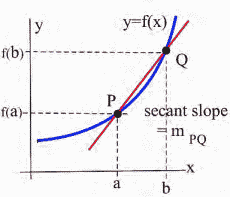
\includegraphics[width=0.24\textwidth]{img/chap2/image111.png}
  %\end{center}
%\vspace{-20pt}  
\caption{Secant line through points $P$ and $Q$}
\label{fig:2-1-secant}
\end{figure}
%\vspace{-10pt}
%\end{wrapfigure}

\begin{definition}
The {\bf rate of change}\index{Rate of change} of a function $f(x)$ between two points, $P = (a, f(a))$ and $Q = (b, f(b))$, on the curve $y=f(x)$ is the slope of the secant line of the curve $y=f(x)$ between the points $P$ and $Q$:
$$\mbox{Rate of change of } f(x) \mbox{ from } a \mbox{ to } b = \mbox{Slope from } P \mbox{ to } Q = \frac{f(b)-f(a)}{b-a} \enspace .$$
\end{definition}

\subsection{Exercises}

\begin{enumerate}
    \item What is the slope of the line between the points $(4, -2)$ and $(7, 10)$?
    \item What is the slope of the line between the points $(-1, 6)$ and $(3, -10)$?
    \item The S\&P 500 rose from \$3244.67 to \$3756.07 in 2020. What is the average rate of change of the S\&P 500 in 2020?
    \item The price of a share of the S\&P 500 ETF SPY rose from \$323.54 to \$373.8 in 2020. What is the average rate of change of a share price of SPY in 2020?
\end{enumerate}

